\documentclass[a3paper]{article}
% \documentclass[a4paper]{article}
\usepackage[margin=1in,centering,includefoot]{geometry}
\usepackage{tikz}
\usetikzlibrary{calendar}

% Taking from https://tex.stackexchange.com/a/10199
\makeatletter%
\tikzoption{day headings}{\tikzstyle{day heading}=[#1]}
\tikzstyle{day heading}=[]
\tikzstyle{day letter headings}=[
    execute before day scope={ \ifdate{day of month=1}{%
      \pgfmathsetlength{\pgf@ya}{\tikz@lib@cal@yshift}%
      \pgfmathsetlength\pgf@xa{\tikz@lib@cal@xshift}%
      \pgftransformyshift{-\pgf@ya}
      \foreach \d/\l in {0/M,1/T,2/W,3/T,4/F,5/S,6/S} {
        \pgf@xa=\d\pgf@xa%
        \pgftransformxshift{\pgf@xa}%
        \pgftransformyshift{3em}%
        \node[every day,day heading]{\l};%
      } 
    }{}%
  }%
]

\makeatother%

\begin{document}
\pagestyle{empty}
\centering
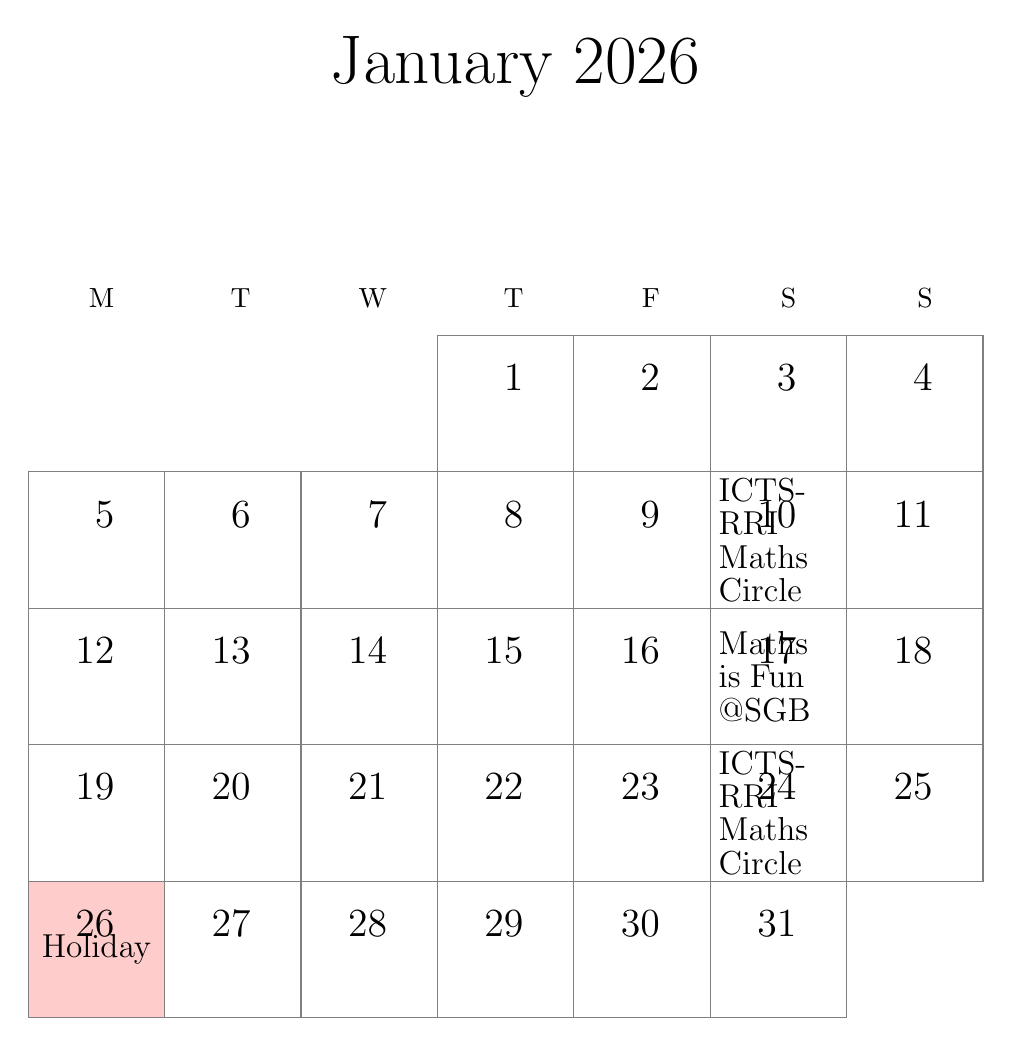
\begin{tikzpicture}
    \calendar [
      name=cal,
        dates=2026-01-01 to 2026-01-last,
        week list,
        day text={\Large\%d-},
        % day text={\%d-},
        day xshift=\textwidth/7,
        day yshift=\textwidth/7,
        month label above centered,
        month text={\Huge {\%mt} \%y-},
        day letter headings
        ]
      if (equals=2026-01-26) {
        \filldraw [red!20] ++({-\textwidth/14-1em},2em) rectangle ++(\textwidth/7,-\textwidth/7) node[pos=.5, align=left, black] {\large Holiday};
      }
      if (equals=\year-\month-08) {
        \draw ++({-\textwidth/14-1em},2em) rectangle ++(\textwidth/7,-\textwidth/7) node[pos=.5, align=left, black, text width=\textwidth/8] {\large ICTS-RRI Maths Circle};
      }
      if (equals=2026-01-10) {
        \draw ++({-\textwidth/14-1em},2em) rectangle ++(\textwidth/7,-\textwidth/7) node[pos=.5, align=left, black, text width=\textwidth/8] {\large ICTS-RRI Maths Circle};
      }
      if (equals=2026-01-17) {
        \draw ++({-\textwidth/14-1em},2em) rectangle ++(\textwidth/7,-\textwidth/7) node[pos=.5, align=left, black, text width=\textwidth/8] {\large Maths is Fun @SGB};
      }
      if (equals=2026-02-07) {
        \draw ++({-\textwidth/14-1em},2em) rectangle ++(\textwidth/7,-\textwidth/7) node[pos=.5, align=left, black, text width=\textwidth/8] {\large Maths is Fun @SGB};
      }
      if (equals=2026-02-21) {
        \draw ++({-\textwidth/14-1em},2em) rectangle ++(\textwidth/7,-\textwidth/7) node[pos=.5, align=left, black, text width=\textwidth/8] {\large Maths is Fun @SGB};
      }
      if (equals=2026-03-07) {
        \draw ++({-\textwidth/14-1em},2em) rectangle ++(\textwidth/7,-\textwidth/7) node[pos=.5, align=left, black, text width=\textwidth/8] {\large Maths is Fun @SGB};
      }
      if (equals=2026-01-24) {
        \draw ++({-\textwidth/14-1em},2em) rectangle ++(\textwidth/7,-\textwidth/7) node[pos=.5, align=left, black, text width=\textwidth/8] {\large ICTS-RRI Maths Circle};
      }
      if (equals=\year-\month-22) {
        \draw ++({-\textwidth/14-1em},2em) rectangle ++(\textwidth/7,-\textwidth/7) node[pos=.5, align=left, black, text width=\textwidth/8] {\large ICTS-RRI Maths Circle};
      }
      if (equals=\year-\month-30) {
        \draw ++({-\textwidth/14-1em},2em) rectangle ++(\textwidth/7,-\textwidth/7) node[pos=.5, align=left, black, text width=\textwidth/8] {\large PriSM};
      }
            if (equals=\year-\month-23) {
        \draw ++({-\textwidth/14-1em},2em) rectangle ++(\textwidth/7,-\textwidth/7) node[pos=.5, align=left, black, text width=\textwidth/8] {\large KwK};
      }
      if (all) {
      \draw[gray] ++({-\textwidth/14-1em},2em) rectangle ++(\textwidth/7,-\textwidth/7);
      };
\end{tikzpicture}
\vspace{\fill}
\section*{Notes}
\vspace{\fill}
\begin{tikzpicture}
  \foreach \i in {1,2,...,5}
    \draw (0,1.25*\i)  -- (0.8*\textwidth,1.25*\i);
\end{tikzpicture}
\end{document}